\chapter{エルミート観測量、スピン、確率規則}

\lectureoverview{量子力学は確率の計算法である。これを理解をスローガンで置き換えることなく用いるには、複素位相、規格化された状態、エルミート観測量、固有値と固有ベクトル、直交性、ボルンの規則という簡潔な数学的連鎖が必要である。三つのパウリ行列は、この連鎖を電子スピンに対する具体的な予言へと変える。}

\section{複素数の極形式}

まず、代数的な摩擦の小さな原因を一つ取り除こう。複素数
\begin{equation}
  z=x+iy
\end{equation}
は複素平面上の点であり、\(x\)は実軸上に、\(y\)は虚軸上にある。この点が極座標\((r,\theta)\)をもつならば、
\begin{equation}
  x=r\cos\theta,
  \qquad
  y=r\sin\theta,
\end{equation}
であり、したがって
\begin{equation}
  z=r(\cos\theta+i\sin\theta)=re^{i\theta}.
  \label{eq:l03-polar-form}
\end{equation}
となる。オイラーの記法が有用なのは、角度の加法定理が指数法則
\begin{equation}
  e^{i\theta}e^{i\phi}
  =e^{i(\theta+\phi)}.
  \label{eq:l03-phase-product}
\end{equation}
になるからである。実際、二つの三角関数形式を掛け合わせると
\begin{align}
& (\cos\theta+i\sin\theta)(\cos\phi+i\sin\phi)
\notag\\
&\qquad=\cos(\theta+\phi)+i\sin(\theta+\phi).
\end{align}
が得られる。よく知られた加法定理はすべてこの一つの掛け算に含まれている。

複素共役は点を実軸に関して折り返す：
\begin{equation}
  z^*=x-iy,
  \qquad
  (e^{i\theta})^*=e^{-i\theta}.
\end{equation}
したがって、
\begin{equation}
  e^{i\theta}e^{-i\theta}=1.
\end{equation}
である。\(e^{i\theta}\)の形の数は単位円上にあり、\emph{純粋位相}と呼ばれる。すべての非零複素数は正の絶対値と純粋位相の積である：
\begin{equation}
  z=|z|e^{i\theta},
  \qquad
  |z|^2=z^*z=x^2+y^2.
  \label{eq:l03-modulus-phase}
\end{equation}

\begin{classroomqa}
\lecturetimestamp{00:06:36}
\audiencequestion{\(\theta\)を\(-\theta\)に変えることは、複素平面における回転の向きを逆にすることに対応するか？}
\lecturerresponse{はい。正と負の位相角は単位円を互いに逆の向きにたどる。複素共役は\(e^{i\theta}\)を\(e^{-i\theta}\)に変えるが、これは折り返された点であり、逆位相である。}
\end{classroomqa}

今日必要とされる複素数の滑走路はこれで全部である：絶対値、位相、共役、そして単位円。

\section{確率の計算法としての量子力学}

次に公理に移る。物理系は\emph{状態}に準備され、測定は\emph{観測量}の値を問い、量子力学は可能な答えに対する確率を与える。

状態は複素ベクトル空間のベクトルである。二準位スピン系に対して、
\begin{equation}
  \ket\psi=\alpha\ket{u}+\beta\ket{d},
  \qquad
  \ket{u}=\begin{pmatrix}1\\0\end{pmatrix},
  \qquad
  \ket{d}=\begin{pmatrix}0\\1\end{pmatrix}.
  \label{eq:l03-two-level-state}
\end{equation}
係数が上向き／下向きの確率を定め、
\begin{equation}
  P(u)=|\alpha|^2,
  \qquad
  P(d)=|\beta|^2,
\end{equation}
したがって状態は規格化されなければならない：
\begin{equation}
  \braket{\psi}{\psi}
  =|\alpha|^2+|\beta|^2
  =1.
  \label{eq:l03-state-normalization}
\end{equation}
次元とは、通常の空間の次元ではなく、状態空間における独立な選択肢の数を指す。三つの互いに排他的な基底状態をもつ系ならば、三つの正規直交列と三つの振幅を用いることになる。

確率は振幅を完全には決定しない。純粋位相を掛けても絶対値は変わらない：
\begin{equation}
  |e^{i\theta}\alpha|^2=|\alpha|^2.
\end{equation}
したがって振幅は、この一つの基底に対する確率を超える情報を含んでいる。その役割は、異なる測定や、後に時間発展を考えるときに明らかになるであろう。

基底状態は正規直交である：
\begin{equation}
  \braket{u}{u}=\braket{d}{d}=1,
  \qquad
  \braket{u}{d}=\braket{d}{u}=0.
\end{equation}
それらの直交性は状態の複素空間に属する。これを通常の三次元空間における直角をなす二つの矢印とまだ混同してはならない。この区別は講義の終わり近くで決定的になるであろう。

\section{なぜ観測量はエルミートなのか}

実験結果は実数として記録できる。便宜上、二つの実数を一つの複素数にまとめてもよいが、指針の読みそのものは常に実量に分離できる。有限次元では、量子観測量は特別なクラスの線形演算子、すなわちエルミート行列によって表される。

それらを定義するために、まず行と列を入れ替えて行列を転置する：
\begin{equation}
  (M^T)_{ij}=M_{ji}.
  \label{eq:l03-transpose}
\end{equation}
\(M^T=M\)を満たす実行列は対称である。複素行列に対する対応する操作はエルミート共役であり、
\begin{equation}
  M^\dagger=(M^T)^*,
  \qquad
  (M^\dagger)_{ij}=M_{ji}^*.
  \label{eq:l03-dagger}
\end{equation}
である。

\begin{figure}[htbp]
\centering
\includegraphics[width=0.88\linewidth]{lecture_03_figure_02.png}
\caption{転置、対称性、そしてエルミート共役への移行は一つの黒板配置を共有している。}
\lectureframe{00:23:06}
\end{figure}

\begin{definition}
行列\(M\)が\emph{エルミート}である条件は、次の等式が成り立つことである。
\begin{equation}
  M^\dagger=M,
  \qquad\text{equivalently}\qquad
  M_{ij}=M_{ji}^*.
  \label{eq:l03-hermitian}
\end{equation}
\end{definition}


対角成分は実である。なぜなら\(M_{ii}=M_{ii}^*\)だからである。折り返された非対角成分は共役対である。したがって一般的な二行二列の形は
\begin{equation}
  M=
  \begin{pmatrix}
    a&z\\
    z^*&b
  \end{pmatrix},
  \qquad a,b\in\mathbb R.
  \label{eq:l03-hermitian-two}
\end{equation}
である。エルミート性は実数条件の行列版であり、すべての成分が個別に実であることを要求するものではない。

最初の成果は二つの初等的な共役恒等式から従う：
\begin{equation}
  \braket{B}{A}=\braket{A}{B}^*,
  \label{eq:l03-inner-conjugation}
\end{equation}
そして、任意の\(M\)に対して、
\begin{equation}
  \bra B M\ket A
  =
  \bigl(\bra A M^\dagger\ket B\bigr)^*.
  \label{eq:l03-matrix-element-conjugation}
\end{equation}
である。式\(\bra B M\ket A\)は数であり、\(M\)の\(BA\)行列要素である。\(M\)がエルミートで\(B=A\)ならば、
\begin{equation}
  \bra A M\ket A
  =
  \bigl(\bra A M\ket A\bigr)^*.
\end{equation}
したがってそれは実である。

\begin{proposition}
すべてのエルミートな\(M\)に対して、期待値
\begin{equation}
  \expect{M}_A=\bra A M\ket A
  \label{eq:l03-expectation}
\end{equation}
はすべての規格化された状態\(\ket A\)において実である。
\end{proposition}

期待値の確率的な意味はさらに展開されるが、その実数性だけでも、なぜエルミート演算子が観測量の自然な候補となるのかがすでに説明される。

\begin{classroomqa}
\lecturetimestamp{00:33:22}
\audiencequestion{平均を表す山括弧の記法は、ブラ--ケット記法に由来するのですか。}
\lecturerresponse{はい。ディラックのブラケット記法は同じ括弧を与えます。\(\bra A M\ket A\)では、演算子が状態を表すブラとケットの間に挟まれ、その結果が期待値となります。}
\end{classroomqa}

\begin{classroomqa}
\lecturetimestamp{00:34:31}
\audiencequestion{物理量そのものが虚数の測定値をもつことはあり得ますか。測定値が実数なら、なぜ量子力学に複素数が必要なのですか。}
\lecturerresponse{測定結果の集合は、たとえその対を一つの複素数としてまとめることを選んだとしても、常に実数として記録できます。より鋭い問いは、なぜ理論が複素振幅へと駆り立てられるのかです。その問いは保留にしてください。答えは可逆な時間発展に関係しており、それはまだ導入されていません。理論を実ベクトルに制限すると、重要な可能性が失われてしまいます。}
\end{classroomqa}

数学は飾りではない。それなしでは、もつれは定義されないまま神秘的に響かせることができてしまう。我々は最も単純な設定、すなわち一つの二準位系で続ける。そうすれば、後にそのような系を二つ、誠実に組み合わせることができる。

\section{固有値は可能な測定結果である}

\begin{definition}
零でないベクトル\(\ket a\)が固有値\(\lambda_a\)をもつ\(M\)の固有ベクトルであるとは、
\begin{equation}
  M\ket a=\lambda_a\ket a.
  \label{eq:l03-eigenvalue-equation}
\end{equation}
を満たすことである。
\end{definition}
行列はベクトルの長さや位相を変え得るが、状態空間においてそれを異なる方向へ変えることはない。

エルミート行列では固有値は実数である。式~\eqref{eq:l03-eigenvalue-equation}の左から\(\bra a\)を掛けると、
\begin{equation}
  \bra a M\ket a
  =\lambda_a\braket{a}{a}.
\end{equation}
が得られる。左辺はエルミート性により実数であり、右辺のノルムは実数で正である。したがって
\begin{equation}
  \lambda_a
  =
  \frac{\bra a M\ket a}{\braket{a}{a}}
  \in\mathbb R.
  \label{eq:l03-real-eigenvalue}
\end{equation}

ここで物理的な主張が来る。\(M\)が観測量を表すとき、その固有値は\(M\)の測定が返し得る値である。\(\lambda_a\)に属する固有ベクトルは、その値が確実に生じる状態である。

最も単純な例は対角行列である。
\begin{equation}
  M=
  \begin{pmatrix}
    m_{11}&0\\
    0&m_{22}
  \end{pmatrix}.
\end{equation}

\begin{figure}[htbp]
\centering
\includegraphics[width=0.72\linewidth]{lecture_03_figure_03.png}
\caption{抽象的な固有値方程式は、最初の対角行列の例の上に置かれている。}
\lectureframe{00:44:04}
\end{figure}

直接の掛け算により
\begin{align}
  M\begin{pmatrix}1\\0\end{pmatrix}
  &=m_{11}\begin{pmatrix}1\\0\end{pmatrix},
  \notag\\
  M\begin{pmatrix}0\\1\end{pmatrix}
  &=m_{22}\begin{pmatrix}0\\1\end{pmatrix}.
  \label{eq:l03-diagonal-eigenvectors}
\end{align}

\begin{figure}[htbp]
\centering
\includegraphics[width=0.72\linewidth]{lecture_03_figure_04.png}
\caption{下側の基底ベクトルは、下側の対角成分を掛けられたものとして返る。}
\lectureframe{00:45:58}
\end{figure}

より大きな対角行列でも同じ規則が成り立つ。その対角成分が固有値であり、標準的なワンホット列が固有ベクトルである。

\section{三つのスピン行列}

第三軸に沿った電子スピンに対しては、
\begin{equation}
  \sigma_3=
  \begin{pmatrix}
    1&0\\
    0&-1
  \end{pmatrix}.
\end{equation}
を選ぶ。その固有状態は、固有値\(+1\)をもつ\(\ket u=(1,0)^T\)と、固有値\(-1\)をもつ\(\ket d=(0,1)^T\)である。したがって、二つの可能な検出器の値はこの二つの固有値である。

第一軸のスピン行列は
\begin{equation}
  \sigma_1=
  \begin{pmatrix}
    0&1\\
    1&0
  \end{pmatrix}.
\end{equation}
である。その候補となる固有ベクトルは、まず規格化せずに書く。固有ベクトルに零でない任意のスカラーを掛けても固有ベクトルのままであるからである。しかし物理的な状態は規格化されなければならない。
\begin{align}
  \ket{x+}
  &=\frac{1}{\sqrt2}\begin{pmatrix}1\\1\end{pmatrix},
  &
  \sigma_1\ket{x+}&=+\ket{x+},
  \notag\\
  \ket{x-}
  &=\frac{1}{\sqrt2}\begin{pmatrix}1\\-1\end{pmatrix},
  &
  \sigma_1\ket{x-}&=-\ket{x-}.
  \label{eq:l03-sigma-one-eigenvectors}
\end{align}

\begin{figure}[htbp]
\centering
\includegraphics[width=0.72\linewidth]{lecture_03_figure_05.png}
\caption{非対角行列と等重みの候補は、積が完成される前に現れる。}
\lectureframe{00:50:29}
\end{figure}

\begin{classroomqa}
\lecturetimestamp{00:56:45}
\audiencequestion{\(\sigma_1\)の固有ベクトルは、代数で求めるのではなく幾何学的に見ることができますか。}
\lecturerresponse{実二成分の描像では、\(\sigma_1\)は基底方向\(E_1\)と\(E_2\)を入れ替える。対角方向\((1,1)^T\)は固定され、もう一方の対角方向\((1,-1)^T\)は反転する。したがってそれらは固有値\(+1\)と\(-1\)をもつ固有ベクトルである。これは成分空間における描像であり、まだ物理的なスピンの指針についての主張ではない。}
\end{classroomqa}

残りの行列は
\begin{equation}
  \sigma_2=
  \begin{pmatrix}
    0&-i\\
    i&0
  \end{pmatrix},
\end{equation}
であり、規格化された固有ベクトルは
\begin{equation}
  \ket{y+}=\frac{1}{\sqrt2}\begin{pmatrix}1\\i\end{pmatrix},
  \qquad
  \ket{y-}=\frac{1}{\sqrt2}\begin{pmatrix}1\\-i\end{pmatrix}.
  \label{eq:l03-sigma-two-eigenvectors}
\end{equation}
である。それらの固有値もまた\(+1\)と\(-1\)である。

三つの行列はすべて二乗すると単位行列になる。
\begin{equation}
  \sigma_1^2=\sigma_2^2=\sigma_3^2=I.
  \label{eq:l03-pauli-squares}
\end{equation}
もし\(\sigma_i\ket a=\lambda\ket a\)ならば、\(\sigma_i\)を二度適用すると\(\lambda^2=1\)が得られるので、\(\lambda=\pm1\)である。この同一のスペクトルは、これらの行列が等価な空間軸に沿ったスピン成分を表すことの最初の兆候である。

\section{異なる結果は直交状態を要求する}

次の定理を証明する前に、その意味を述べる。もし一つの観測量がある状態と別の状態で二つの異なる確定した答えを与えるなら、その観測量の測定はそれらの状態を完全に区別できる。量子力学はこの完全な区別可能性を直交性として表す。

\begin{theorem}
\(M\) をエルミートとし、
\begin{equation}
  M\ket A=\lambda_A\ket A,
  \qquad
  M\ket B=\lambda_B\ket B.
\end{equation}
\(\lambda_A\ne\lambda_B\) ならば、
\begin{equation}
  \braket{B}{A}=0.
\end{equation}
\end{theorem}

\begin{proof}
最初の固有値方程式に \(\bra B\) を掛けると
\begin{equation}
  \bra B M\ket A=\lambda_A\braket{B}{A}.
\end{equation}
が得られる。エルミート性と第二の固有値方程式により、同じ行列要素は
\begin{equation}
  \bra B M\ket A=\lambda_B\braket{B}{A},
\end{equation}
となる。なぜなら \(\lambda_B\) は実数だからである。差を取ると
\begin{equation}
  (\lambda_A-\lambda_B)\braket{B}{A}=0.
\end{equation}
となる。固有値は異なるので、内積はゼロでなければならない。
\end{proof}

\(\sigma_1\) の固有ベクトルは即座に確認を与える：
\begin{equation}
  \braket{x+}{x-}
  =
  \frac12
  \begin{pmatrix}1&1\end{pmatrix}
  \begin{pmatrix}1\\-1\end{pmatrix}
  =\frac12-\frac12=0.
\end{equation}
逆に、二つの直交する状態に対しては、それらを区別する測定が存在する。したがって直交性は単なる幾何学的な言葉ではなく、操作的な意味を持つ。

\section{確率の公準}

系が規格化された状態 \(\ket B\) に準備されているとする。\(M\) を可観測量とし、\(\ket A\) を固有値 \(\lambda_A\) を持つ \(M\) の規格化された固有ベクトルとする。このとき、\(M\) を測定して \(\lambda_A\) が得られる確率は
\begin{equation}
  P(\lambda_A\mid B)
  =
  |\braket{A}{B}|^2
  =
  \braket{A}{B}\braket{B}{A}.
  \label{eq:l03-born-rule}
\end{equation}
である。この積は実数かつ非負である。規格化されたベクトルに対しては、それは高々1である。

\begin{figure}[htbp]
\centering
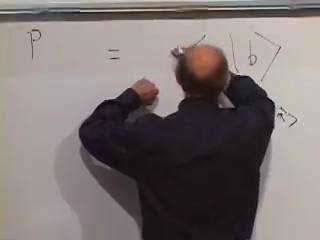
\includegraphics[width=0.78\linewidth]{lecture_03_figure_06.png}
\caption{確率規則は、重なりとその複素共役との積として書かれる。}
\lectureframe{01:16:40}
\end{figure}

\begin{classroomqa}
\lecturetimestamp{01:19:19}
\audiencequestion{これは二つの状態の間の角度の余弦の二乗だろうか？}
\lecturerresponse{通常のユークリッド空間における実単位ベクトルに対しては、内積は角度の余弦である。ここでは内積は一般に複素数であるから、その余弦となる通常の空間的な角度は存在しない。有用な類似物は重なりの大きさであり、確率はその絶対値の二乗である。}
\end{classroomqa}

\begin{classroomqa}
\lecturetimestamp{01:20:18}
\audiencequestion{準備された状態が、\(M\) の異なる固有値を持つ別の固有ベクトルである場合はどうか？}
\lecturerresponse{そのとき、二つの固有ベクトルは直交する。それらの重なりはゼロであるから、\(\lambda_A\) を得る確率はゼロである。一つの確定した値を持つ状態を準備することは、同じ可観測量の異なる確定した値を排除する。}
\end{classroomqa}

\begin{classroomqa}
\lecturetimestamp{01:21:23}
\audiencequestion{どの結果も確実でないような準備を、同じ規則で扱えるだろうか？}
\lecturerresponse{はい。それが一般的な場合である：\(\ket B\) は \(M\) の固有状態である必要はない。規格化された固有ベクトルとの重なりが、対応する結果の確率を与える。より複雑な分布を扱う前に、まず二つの結果を持つ例から始めている。}
\end{classroomqa}

この講義は、規則を一つの式の中に隠すのではなく、いくつかの準備状態に対して訓練する。

まず \(\sigma_3=+1\) を準備する：
\begin{equation}
  \ket B=\ket{u}=\begin{pmatrix}1\\0\end{pmatrix}.
\end{equation}
\(\sigma_1\) を測定する。その \(+1\) 固有ベクトルに対して、
\begin{equation}
  \braket{x+}{u}
  =
  \frac{1}{\sqrt2}
  \begin{pmatrix}1&1\end{pmatrix}
  \begin{pmatrix}1\\0\end{pmatrix}
  =\frac{1}{\sqrt2},
\end{equation}
したがって
\begin{equation}
  P(\sigma_1=+1\mid\sigma_3=+1)=\frac12.
\end{equation}
\(\ket{x+}\) を \(\ket{x-}\) に置き換えても同じ確率が得られる。準備と測定を逆にしても、重なりの絶対値の二乗は対称であるから、やはり二分の一が得られる。

真に複素数の例として、\(\ket{x+}\) を準備し、\(\sigma_2\) を測定する。このとき
\begin{align}
  \braket{y+}{x+}
  &=
  \frac12
  \begin{pmatrix}1&-i\end{pmatrix}
  \begin{pmatrix}1\\1\end{pmatrix}
  =\frac{1-i}{2},
  \notag\\
  P(\sigma_2=+1\mid\sigma_1=+1)
  &=\left|\frac{1-i}{2}\right|^2
  =\frac14+\frac14
  =\frac12.
  \label{eq:l03-complex-probability-example}
\end{align}
したがって、ある軸に沿ってスピンを準備し、垂直な軸に沿って測定すると、二つの結果に対して等しい確率が得られる。

\section{ポインター、状態、任意の軸}

前の文は、用語を修正しないと誤解されうる。磁気モーメントは空間的な向きを持ち、これを \emph{ポインター} と呼ぶことにする。ケットは複素状態空間のベクトルである。二つの空間的ポインターは垂直でありうるが、二つの状態ベクトルは直交しうる。これらは異なる空間における異なる主張である。

\begin{classroomqa}
\lecturetimestamp{01:29:25}
\audiencequestion{二つの物理的なスピンの向きが九十度離れているなら、それらの状態ベクトルは直交すべきだろうか？}
\lecturerresponse{いいえ。垂直な空間軸に沿ったスピンアップ状態は、重なりの二乗が \(1/2\) であり、ゼロではない。ある軸に沿ったスピンアップに直交する状態は、同じ軸に沿ったスピンダウンである。\emph{垂直} は通常の空間におけるポインターのために、\emph{直交} は完全に区別可能な状態のために取っておく。}
\end{classroomqa}

\begin{classroomqa}
\lecturetimestamp{01:31:25}
\audiencequestion{\emph{独立}を\emph{直交}の代わりに使うことはできますか。}
\lecturerresponse{いいえ。線形独立は、どのベクトルも他のベクトルのスカラー倍ではないということだけを述べており、内積がゼロであることを要求するものではありません。直交性はより強い条件であり、ここでは完全な識別可能性という物理的意味を持ちます。}
\end{classroomqa}

\(\hat n=(n_1,n_2,n_3)\) を通常の空間における単位ポインターとする：
\begin{equation}
  n_1^2+n_2^2+n_3^2=1.
\end{equation}
その方向に沿ったスピンの演算子は、内積の行列値類似物である：
\begin{equation}
  \boldsymbol{\sigma}\cdot\hat n
  =
  n_1\sigma_1+n_2\sigma_2+n_3\sigma_3
  =
  \begin{pmatrix}
    n_3&n_1-in_2\\
    n_1+in_2&-n_3
  \end{pmatrix}.
  \label{eq:l03-spin-arbitrary-axis}
\end{equation}
それはエルミートである：対角成分は実数であり、非対角成分は複素共役である。

\begin{figure}[htbp]
\centering
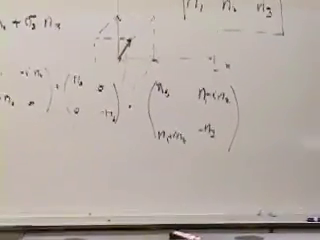
\includegraphics[width=0.84\linewidth]{lecture_03_figure_07.png}
\caption{空間単位ポインタ、演算子の和、およびその明示的なエルミート行列をまとめて展開する。}
\lectureframe{01:38:00}
\end{figure}

その取り得る値を求めるには、行列要素を代入する前に対数を二乗する。行列の順序が重要であるため、交差項は反交換子として現れる：
\begin{align}
  (\boldsymbol{\sigma}\cdot\hat n)^2
  &=
  n_1^2\sigma_1^2+n_2^2\sigma_2^2+n_3^2\sigma_3^2
  \notag\\
  &\quad
  +n_1n_2(\sigma_1\sigma_2+\sigma_2\sigma_1)
  \notag\\
  &\quad
  +n_2n_3(\sigma_2\sigma_3+\sigma_3\sigma_2)
  \notag\\
  &\quad
  +n_1n_3(\sigma_1\sigma_3+\sigma_3\sigma_1).
  \label{eq:l03-axis-square-expanded}
\end{align}
異なるパウリ行列は反交換する：
\begin{equation}
  \sigma_i\sigma_j+\sigma_j\sigma_i=0
  \qquad(i\ne j).
  \label{eq:l03-pauli-anticommutation}
\end{equation}
講義では一つの場合を明示的に確認する：
\begin{equation}
  \sigma_1\sigma_3
  =
  \begin{pmatrix}0&-1\\1&0\end{pmatrix},
  \qquad
  \sigma_3\sigma_1
  =
  \begin{pmatrix}0&1\\-1&0\end{pmatrix}
  =-\sigma_1\sigma_3.
  \label{eq:l03-order-check}
\end{equation}

\begin{figure}[htbp]
\centering
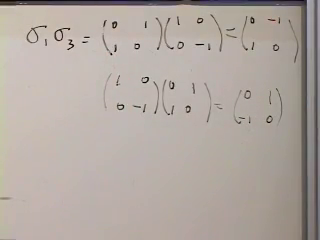
\includegraphics[width=0.82\linewidth]{lecture_03_figure_08.png}
\caption{\(\sigma_1\) と \(\sigma_3\) を逆の順序で掛けると、符号が異なる行列が得られる。}
\lectureframe{01:44:50}
\end{figure}

式~\eqref{eq:l03-axis-square-expanded}の交差項は消え、一方で \(\sigma_i^2=I\) である。したがって
\begin{equation}
  (\boldsymbol{\sigma}\cdot\hat n)^2
  =(n_1^2+n_2^2+n_3^2)I
  =I.
\end{equation}
すべての固有値は \(\lambda^2=1\) を満たす：
\begin{equation}
  \lambda=\pm1.
\end{equation}
装置がどの空間軸を選んでも、検出器には依然として \(+1\) と \(-1\) の二つの結果しかない。近接する方向の関係は中間の測定値として現れるのではなく、これら二つの固定された答えの確率の中に現れる。
